\newif\ifsolutions
\solutionstrue % Show solutions
%\solutionsfalse % Hide solutions

\documentclass{article}
\usepackage{geometry}
\geometry{margin=1in}
\usepackage{tikz}
\usepackage{amssymb}

% fleqn allows setting indent of display math
\usepackage[fleqn]{amsmath}
\setlength{\mathindent}{0pt} % Set indent
% Disable equation numbering (https://tex.stackexchange.com/a/360378)
\makeatletter
\renewcommand\tagform@[1]{}
\makeatother

% Allow Unicode (some, e.g., © and £ at least)
% https://tex.stackexchange.com/questions/370278/is-there-any-reason-to-use-inputenc
\usepackage[utf8]{inputenc}

% Hyperlinks
\usepackage{hyperref}
\hypersetup{colorlinks=true, urlcolor=blue, linkcolor=blue}

% Prevent indentation of paragraphs
\setlength\parindent{0pt}
\setlength{\parskip}{\baselineskip}

% Spacing above/below equations
% https://tex.stackexchange.com/a/69678
\AtBeginDocument{%
 \abovedisplayskip=-\parskip
 \abovedisplayshortskip=-\parskip
 \belowdisplayskip=0pt
 \belowdisplayshortskip=0pt
}

% Allow 3 additional subsection levels
% https://tex.stackexchange.com/a/60212
\usepackage{titlesec}
\setcounter{secnumdepth}{6}
% H4 in HTML
\titleformat{\paragraph}{\normalfont\normalsize\bfseries}{\theparagraph}{1em}{}
\titlespacing*{\paragraph}{0pt}{3.25ex plus 1ex minus .2ex}{1.5ex plus .2ex}
% H5 in HTML
\titleformat{\subparagraph}{\normalfont\normalsize\bfseries}{\thesubparagraph}{1em}{}
\titlespacing*{\subparagraph}{0pt}{3.25ex plus 1ex minus .2ex}{1.5ex plus .2ex}
% H6 in HTML
\titleformat{\subsubparagraph}{\normalfont\normalsize\bfseries}{\thesubsubparagraph}{1em}{}
\titlespacing*{\subsubparagraph}{0pt}{3.25ex plus 1ex minus .2ex}{1.5ex plus .2ex}

% So enumerate at all levels is numbers
% https://tex.stackexchange.com/questions/78842/nested-enumeration-numbering
\renewcommand{\labelenumii}{\arabic{enumii}.}
\renewcommand{\labelenumiii}{\arabic{enumiii}.}
\renewcommand{\labelenumiv}{\arabic{enumiv}.}

\renewcommand{\mbox}{\text}
\newcommand{\ds}[0]{\displaystyle}
\newcommand{\ihat}[0]{\hat{\boldsymbol{\imath}}}
\newcommand{\jhat}[0]{\hat{\boldsymbol{\jmath}}}
\newcommand{\khat}[0]{\hat{\boldsymbol{k}}}
\newcommand{\xhat}[0]{\hat{\mathbf{x}}}
\newcommand{\yhat}[0]{\hat{\mathbf{y}}}
\newcommand{\zhat}[0]{\hat{\mathbf{z}}}
\newcommand{\rhat}[0]{\hat{\mathbf{r}}}
\newcommand{\bfvec}[1]{\vec{\mathbf{#1}}}
\newcommand{\bfcdot}[0]{\boldsymbol{\cdot}}

\usepackage{fancyhdr}
\pagestyle{fancy}
\lhead{RC Circuits}
\rhead{\thepage}
\fancyfoot{}

\begin{document}

\section{Notation and Equations}

\begin{itemize}

  \item We use the the letter ``C" as a label for a capacitor and the units of charge. When used as a label, $C$ is usually written in itallics. Thus

        ``$Q_C= 10 \text{ C}$" means ``the capacitor labeled $C$ has a charge of $10$ Coulombs."

  \item Lower case letters are used for electrical quantities that vary in time. In circuits with only emfs and resistors, currents and voltages are constant, and we used $I$ and $V$. In the circuits considered in this activity, the currents and voltages vary in time, so we use $i(t)$ and $v(t)$.

  \item In this activity, we use the the relationship $i(t)=dq(t)/dt$ between the current $i(t)$ in the wires connected to a capacitor and the charge $q(t)$ on the capacitor.

\end{itemize}

\section{Discharging Capacitor}

If one capacitor with capacitance $C$ is in a circuit with other resistors (and no emfs), the charge on the capacitor changes with time according to

$q(t)=Q_oe^{-t/\tau}$,

where $\tau\equiv RC$, $Q_o$ is the charge on the capacitor at $t=0$, and $R$ is the equivalent resistance. The quantity $\tau$ is called ``RC time constant." The equation for $q(t)$ follows from using Kirchhoff's voltage law, which gives a differential equation, and then solving the differential equation.

\subsection{Problem}

Find $\tau$ for the following two circuits. Use $R=10\text{ k}\Omega$ and $C=1\text{ }\mu\text{F}$.



\tikzset{every picture/.style={line width=0.75pt}} %set default line width to 0.75pt        

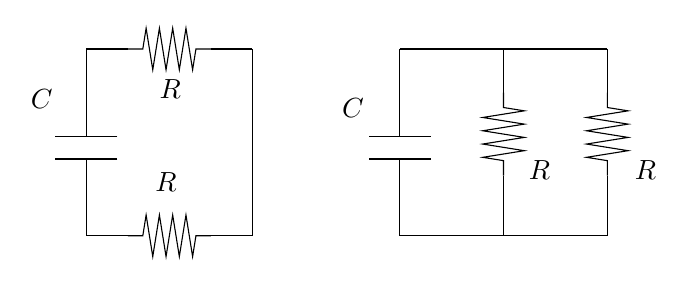
\begin{tikzpicture}[x=0.75pt,y=0.75pt,yscale=-1,xscale=1]
%uncomment if require: \path (0,122); %set diagram left start at 0, and has height of 122

%Shape: Resistor [id:dp05500381774764507] 
\draw   (69,20) -- (76.2,20) -- (77.8,10) -- (81,30) -- (84.2,10) -- (87.4,30) -- (90.6,10) -- (93.8,30) -- (97,10) -- (100.2,30) -- (101.8,20) -- (109,20) ;
%Straight Lines [id:da7355678714340006] 
\draw    (109,20) -- (129,20) ;
%Straight Lines [id:da527045155276259] 
\draw    (129,80) -- (129,110) ;
%Shape: Resistor [id:dp3594116450407856] 
\draw   (69,110) -- (76.2,110) -- (77.8,100) -- (81,120) -- (84.2,100) -- (87.4,120) -- (90.6,100) -- (93.8,120) -- (97,100) -- (100.2,120) -- (101.8,110) -- (109,110) ;
%Straight Lines [id:da9970092949559268] 
\draw    (109,110) -- (129,110) ;
%Straight Lines [id:da3476278762101743] 
\draw    (49,20) -- (69,20) ;
%Straight Lines [id:da4620337269837471] 
\draw    (49,110) -- (69,110) ;
%Straight Lines [id:da9993276379137561] 
\draw    (49,20) -- (49,54.33) ;
%Straight Lines [id:da14261766387593622] 
\draw    (129,20) -- (129,80) ;
%Shape: Contact [id:dp6430887579633948] 
\draw   (49,54.33) -- (49,62.33) (49,81) -- (49,73) (64,62.33) -- (34,62.33) (64,73) -- (34,73) ;
%Straight Lines [id:da5144443528570377] 
\draw    (49,81) -- (49,110) ;
%Shape: Resistor [id:dp9803823329759065] 
\draw   (250,41) -- (250,48.2) -- (260,49.8) -- (240,53) -- (260,56.2) -- (240,59.4) -- (260,62.6) -- (240,65.8) -- (260,69) -- (240,72.2) -- (250,73.8) -- (250,81) ;
%Straight Lines [id:da7114935485860634] 
\draw    (200,20) -- (300,20) ;
%Straight Lines [id:da5684648483404737] 
\draw    (200,110) -- (300,110) ;
%Straight Lines [id:da8213220787595459] 
\draw    (200,20) -- (200,54.33) ;
%Shape: Contact [id:dp09002842999214056] 
\draw   (200,54.33) -- (200,62.33) (200,81) -- (200,73) (215,62.33) -- (185,62.33) (215,73) -- (185,73) ;
%Straight Lines [id:da532030432993386] 
\draw    (200,81) -- (200,110) ;
%Straight Lines [id:da10367742610474684] 
\draw    (250,81) -- (250,110) ;
%Straight Lines [id:da011328159933985171] 
\draw    (250,20) -- (250,48.2) ;
%Shape: Resistor [id:dp8997079321456452] 
\draw   (300,41) -- (300,48.2) -- (310,49.8) -- (290,53) -- (310,56.2) -- (290,59.4) -- (310,62.6) -- (290,65.8) -- (310,69) -- (290,72.2) -- (300,73.8) -- (300,81) ;
%Straight Lines [id:da9942687754475996] 
\draw    (300,81) -- (300,110) ;
%Straight Lines [id:da5427177633185147] 
\draw    (300,20) -- (300,48.2) ;

% Text Node
\draw (83,33.4) node [anchor=north west][inner sep=0.75pt]    {$R$};
% Text Node
\draw (81,78.4) node [anchor=north west][inner sep=0.75pt]    {$R$};
% Text Node
\draw (21,38.4) node [anchor=north west][inner sep=0.75pt]    {$C$};
% Text Node
\draw (312,72.4) node [anchor=north west][inner sep=0.75pt]    {$R$};
% Text Node
\draw (261,72.4) node [anchor=north west][inner sep=0.75pt]    {$R$};
% Text Node
\draw (171,42.4) node [anchor=north west][inner sep=0.75pt]    {$C$};


\end{tikzpicture}


\ifsolutions
\textbf{Answer}:

    \begin{itemize}

      \item Left: $R_{\text{eq}}=20\text{ k}\Omega$; $\tau = R_{\text{eq}}C = (20\cdot 10^3\text{ }\Omega) \cdot (10^{-6}\text{ F}) = 0.02\text{ s}$

      \item Right: $R_{\text{eq}}=5\text{ k}\Omega$; $\tau=.005\text{ s}$

    \end{itemize}
\else
\vskip 72pt
\fi
\ifsolutions\else
\vskip 72pt
\fi

\newpage

\subsection{Problem}

For the following circuit, find the charge $q$ on the capacitor at $t=2\text{ s}$ if the switch is closed at $t=0$ and the capacitor has an initial charge of $Q_o$ for the following three cases.

\begin{enumerate}

  \item $RC=1\text{ s}\qquad$ $q(2\text{ s})=\fbox{\qquad\phantom M}$

  \item $RC=2\text{ s}\qquad$ $q(2\text{ s})=\fbox{\qquad\phantom M}$

  \item $RC=4\text{ s}\qquad$ $q(2\text{ s})=\fbox{\qquad\phantom M}$

\end{enumerate}

\ifsolutions

\else
\vskip 56.25pt
\fi
\ifsolutions\else
\vskip 56.25pt
\fi

Next, sketch a plot of $q(t)$ from $t=0$ to $t=6\text{ s}$ for each of these three cases. Used a solid, dashed, and dotted line for case 1., 2., and 3., respectively.



\tikzset{every picture/.style={line width=0.75pt}} %set default line width to 0.75pt        

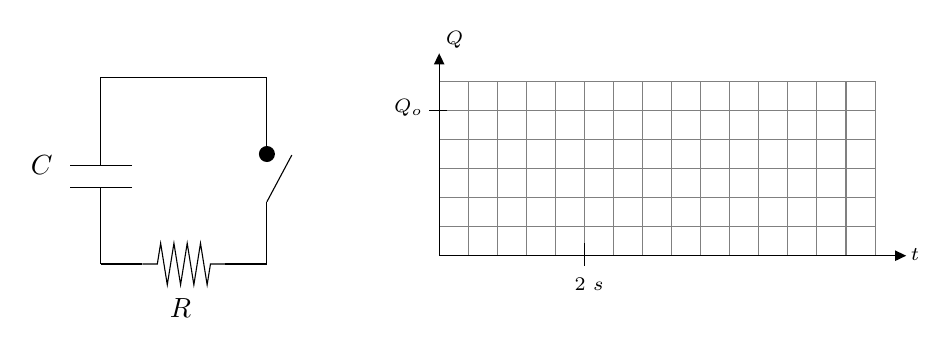
\begin{tikzpicture}[x=0.75pt,y=0.75pt,yscale=-1,xscale=1]
%uncomment if require: \path (0,165); %set diagram left start at 0, and has height of 165

%Straight Lines [id:da21694403558430375] 
\draw    (63,34) -- (123,34) ;
%Straight Lines [id:da12186668018741531] 
\draw    (123,94) -- (123,124) ;
%Shape: Resistor [id:dp5192799178559] 
\draw   (63,124) -- (70.2,124) -- (71.8,114) -- (75,134) -- (78.2,114) -- (81.4,134) -- (84.6,114) -- (87.8,134) -- (91,114) -- (94.2,134) -- (95.8,124) -- (103,124) ;
%Straight Lines [id:da4064606371405326] 
\draw    (103,124) -- (123,124) ;
%Straight Lines [id:da6092949468165629] 
\draw    (43,34) -- (63,34) ;
%Straight Lines [id:da3996966582016197] 
\draw    (43,124) -- (63,124) ;
%Straight Lines [id:da8432524402003263] 
\draw    (43,34) -- (43,68.33) ;
%Straight Lines [id:da5673924877628735] 
\draw    (135,71.5) -- (123,94) ;
%Straight Lines [id:da40110239263509695] 
\draw    (123,34) -- (123,71) ;
\draw [shift={(123,71)}, rotate = 90] [color={rgb, 255:red, 0; green, 0; blue, 0 }  ][fill={rgb, 255:red, 0; green, 0; blue, 0 }  ][line width=0.75]      (0, 0) circle [x radius= 3.35, y radius= 3.35]   ;
%Shape: Contact [id:dp4210243094531454] 
\draw   (43,68.33) -- (43,76.33) (43,95) -- (43,87) (58,76.33) -- (28,76.33) (58,87) -- (28,87) ;
%Straight Lines [id:da39304851837883903] 
\draw    (43,95) -- (43,124) ;
%Shape: Grid [id:dp4136213731791418] 
\draw  [draw opacity=0] (206,36) -- (416,36) -- (416,120) -- (206,120) -- cycle ; \draw  [color={rgb, 255:red, 128; green, 128; blue, 128 }  ,draw opacity=1 ] (206,36) -- (206,120)(220,36) -- (220,120)(234,36) -- (234,120)(248,36) -- (248,120)(262,36) -- (262,120)(276,36) -- (276,120)(290,36) -- (290,120)(304,36) -- (304,120)(318,36) -- (318,120)(332,36) -- (332,120)(346,36) -- (346,120)(360,36) -- (360,120)(374,36) -- (374,120)(388,36) -- (388,120)(402,36) -- (402,120)(416,36) -- (416,120) ; \draw  [color={rgb, 255:red, 128; green, 128; blue, 128 }  ,draw opacity=1 ] (206,36) -- (416,36)(206,50) -- (416,50)(206,64) -- (416,64)(206,78) -- (416,78)(206,92) -- (416,92)(206,106) -- (416,106)(206,120) -- (416,120) ; \draw  [color={rgb, 255:red, 128; green, 128; blue, 128 }  ,draw opacity=1 ]  ;
%Straight Lines [id:da6371695008603995] 
\draw [color={rgb, 255:red, 128; green, 128; blue, 128 }  ,draw opacity=1 ]   (206,120) -- (416,120) ;
%Straight Lines [id:da19392406724359912] 
\draw [color={rgb, 255:red, 128; green, 128; blue, 128 }  ,draw opacity=1 ]   (416,120) -- (416,36) ;

%Straight Lines [id:da5115200356999086] 
\draw    (206,25.5) -- (206,120) ;
\draw [shift={(206,22.5)}, rotate = 90] [fill={rgb, 255:red, 0; green, 0; blue, 0 }  ][line width=0.08]  [draw opacity=0] (5.36,-2.57) -- (0,0) -- (5.36,2.57) -- cycle    ;
%Straight Lines [id:da04281112255200381] 
\draw [color={rgb, 255:red, 0; green, 0; blue, 0 }  ,draw opacity=1 ]   (206,120) -- (428,120) ;
\draw [shift={(431,120)}, rotate = 180] [fill={rgb, 255:red, 0; green, 0; blue, 0 }  ,fill opacity=1 ][line width=0.08]  [draw opacity=0] (5.36,-2.57) -- (0,0) -- (5.36,2.57) -- cycle    ;
%Straight Lines [id:da19821580998780153] 
\draw    (276,114) -- (276,125) ;
%Straight Lines [id:da5919180085071085] 
\draw    (210,50) -- (201,50) ;

% Text Node
\draw (75,139.4) node [anchor=north west][inner sep=0.75pt]    {$R$};
% Text Node
\draw (8,70.4) node [anchor=north west][inner sep=0.75pt]    {$C$};
% Text Node
\draw (208,10.4) node [anchor=north west][inner sep=0.75pt]  [font=\scriptsize]  {$Q$};
% Text Node
\draw (432,115.4) node [anchor=north west][inner sep=0.75pt]  [font=\scriptsize]  {$t$};
% Text Node
\draw (270,129.4) node [anchor=north west][inner sep=0.75pt]  [font=\scriptsize]  {$2\ s$};
% Text Node
\draw (183,43.4) node [anchor=north west][inner sep=0.75pt]  [font=\scriptsize]  {$Q_{o}$};


\end{tikzpicture}


\ifsolutions
\textbf{Answer}:

$q(2)=Q_oe^{-2/RC}$, assuming $RC$ has units of seconds. So

    \begin{enumerate}

      \item $q(2)=Q_oe^{-2/1}=Q_o/e^2 \simeq 0.14 Q_o$

      \item $q(2)=Q_oe^{-2/2}=Q_o/e \simeq 0.37 Q_o$

      \item $q(2)=Q_oe^{-2/4}=Q_o/\sqrt{e} \simeq 0.61 Q_o$

    \end{enumerate}

All curves decay exponentially. To plot, start at $Q_o$, and draw an exponentially decaying curve that passes through one of the values above at $t=2$.
\fi

\subsection{Problem}



\tikzset{every picture/.style={line width=0.75pt}} %set default line width to 0.75pt        

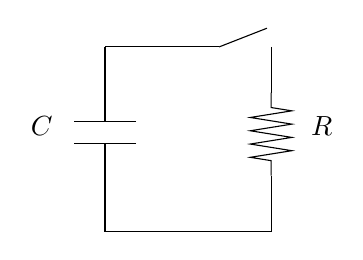
\begin{tikzpicture}[x=0.75pt,y=0.75pt,yscale=-1,xscale=1]
%uncomment if require: \path (0,123); %set diagram left start at 0, and has height of 123

%Shape: Resistor [id:dp627469502609658] 
\draw   (123,42) -- (123,49.2) -- (133,50.8) -- (113,54) -- (133,57.2) -- (113,60.4) -- (133,63.6) -- (113,66.8) -- (133,70) -- (113,73.2) -- (123,74.8) -- (123,82) ;
%Straight Lines [id:da93035776440669] 
\draw    (123,20) -- (123,42) ;
%Straight Lines [id:da18862951458062072] 
\draw    (43,20) -- (98,20) ;
%Straight Lines [id:da26212312116112235] 
\draw    (123,82) -- (123,109) ;
%Straight Lines [id:da2925845653343082] 
\draw    (43,20) -- (43,48) ;
%Shape: Contact [id:dp8830997237938567] 
\draw   (43,48) -- (43,56) (43,74.67) -- (43,66.67) (58,56) -- (28,56) (58,66.67) -- (28,66.67) ;
%Straight Lines [id:da48642353717206155] 
\draw    (43,74.67) -- (43,109) ;
%Straight Lines [id:da4341489184539029] 
\draw    (43,109) -- (123,109) ;
%Straight Lines [id:da7775237515847642] 
\draw    (98,20) -- (121,11) ;

% Text Node
\draw (141,52.4) node [anchor=north west][inner sep=0.75pt]    {$R$};
% Text Node
\draw (6,52.4) node [anchor=north west][inner sep=0.75pt]    {$C$};


\end{tikzpicture}


In the circuit above, the values of $R$ and $C$ are such that $RC=1\text{ s}$.

\begin{enumerate}

  \item If the capacitor has a charge of $10\text{ nC}$ and the switch is closed, how long will it take for the charge on the capacitor to fall to half of this value?

  \item If the capacitor instead had a charge of $20\text{ nC}$ and the switch is closed, how long will it take for the charge on the capacitor to fall to half of this value?

\end{enumerate}

\ifsolutions
\textbf{Answer}:

$q(t)=Q_oe^{-t/\tau}$ and we want $t$ when $q(t)=Q_o/2$, so need to solve 

$Q_o/2=Q_oe^{-t/\tau}\quad$ or $\quad 1/2=e^{-t/\tau}$

Taking the natural log of boths sides, and using $\ln(1/x)=-\ln x$, gives

\begin{equation}
-\ln(2) = \ln e^{-t/\tau} = -\frac{t}{\tau}
\end{equation}

so $t=\tau\ln(2)\simeq 0.70\tau$. The answer does not depend on $Q_o$, so this is the answer for parts 1. and 2.
\else

\newpage
\fi
\ifsolutions\else
\newpage
\fi

\section{Charging a Capacitor}

If a single capacitor is in series with other resistors and a DC voltage source, the charge of the capacitor varies according to 

\begin{equation}
q(t)=Q_f(1-e^{-t/\tau})
\end{equation}

where $\tau\equiv RC$, $R$ is the equivalent resistance, and $Q_f$ is the final charge on the capacitor, that is, the charge on the capacitor as $t\rightarrow\infty$ (it is technically more accurate to say $t\gg \tau$ instead of $t\rightarrow\infty$).

To find $Q_f$, replace the capacitor with an open circuit and use Kirchhoff's voltage law to find the voltage across the capacitor, $V_f$. Then use $Q_f=CV_f$.

\subsection{Example}

Find $q(t)$ for the following circuit, assuming the switch is closed at $t=0$ and the capacitor is initially uncharged.



\tikzset{every picture/.style={line width=0.75pt}} %set default line width to 0.75pt        

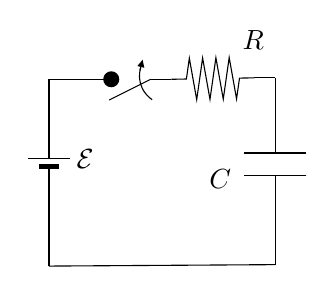
\begin{tikzpicture}[x=0.75pt,y=0.75pt,yscale=-1,xscale=1]
%uncomment if require: \path (0,127); %set diagram left start at 0, and has height of 127

%Straight Lines [id:da6882148732568387] 
\draw    (31,120) -- (139.99,119.3) ;
%Shape: Contact [id:dp12870625792572832] 
\draw   (139.99,57.5) -- (139.99,65.5) (139.99,84.17) -- (139.99,76.17) (154.99,65.5) -- (124.99,65.5) (154.99,76.17) -- (124.99,76.17) ;
%Straight Lines [id:da9572970149113156] 
\draw    (31,71) -- (31,120) ;
%Straight Lines [id:da6113677612125412] 
\draw    (31,30) -- (61,30) ;
\draw [shift={(61,30)}, rotate = 0] [color={rgb, 255:red, 0; green, 0; blue, 0 }  ][fill={rgb, 255:red, 0; green, 0; blue, 0 }  ][line width=0.75]      (0, 0) circle [x radius= 3.35, y radius= 3.35]   ;
%Shape: Resistor [id:dp5166523527809854] 
\draw   (90,30) -- (97.2,29.87) -- (98.62,19.85) -- (102.17,39.79) -- (105.02,19.74) -- (108.57,39.68) -- (111.42,19.62) -- (114.97,39.57) -- (117.82,19.51) -- (121.37,39.45) -- (122.8,29.43) -- (129.99,29.3) ;
%Straight Lines [id:da48829703300868066] 
\draw    (139.99,84.17) -- (139.99,119.3) ;
%Straight Lines [id:da4939203891912127] 
\draw    (139.99,29.3) -- (139.99,57.5) ;
%Straight Lines [id:da8853270867045042] 
\draw    (80,30) -- (90,30) ;
%Straight Lines [id:da940777352086771] 
\draw    (129.99,29.3) -- (139.99,29.3) ;
%Straight Lines [id:da6892602005997428] 
\draw    (21,68) -- (41,68) ;
%Straight Lines [id:da8250911923180322] 
\draw [line width=1.5]    (26,72) -- (36,72) ;
%Straight Lines [id:da863850682244607] 
\draw    (31,30) -- (31,68) ;
%Straight Lines [id:da8715554256964051] 
\draw    (80,30) -- (60,40) ;
%Shape: Arc [id:dp5351289419953953] 
\draw  [draw opacity=0] (80.71,39.82) .. controls (78.71,38.49) and (77.02,36.61) .. (75.91,34.27) .. controls (74.42,31.12) and (74.22,27.68) .. (75.11,24.57) -- (88.36,28.36) -- cycle ; \draw   (80.71,39.82) .. controls (78.71,38.49) and (77.02,36.61) .. (75.91,34.27) .. controls (74.42,31.12) and (74.22,27.68) .. (75.11,24.57) ;  
%Straight Lines [id:da5237669991331495] 
\draw    (75.38,23.48) -- (74.83,25.71) ;
\draw [shift={(76.11,20.57)}, rotate = 104] [fill={rgb, 255:red, 0; green, 0; blue, 0 }  ][line width=0.08]  [draw opacity=0] (3.57,-1.72) -- (0,0) -- (3.57,1.72) -- cycle    ;

% Text Node
\draw (123,5.4) node [anchor=north west][inner sep=0.75pt]    {$R$};
% Text Node
\draw (107,72.4) node [anchor=north west][inner sep=0.75pt]    {$C$};
% Text Node
\draw (43,62.4) node [anchor=north west][inner sep=0.75pt]    {$\mathcal{E}$};


\end{tikzpicture}


\textbf{Answer}: When the switch is closed, charge builds up on the capacitor. This build--up continues until the charge on the capacitor is such that no current flows in the circuit. If no current flows through the capacitor, the circuit is equivalent to one in which the capacitor is replaced with an open circuit, as shown below. 



\tikzset{every picture/.style={line width=0.75pt}} %set default line width to 0.75pt        

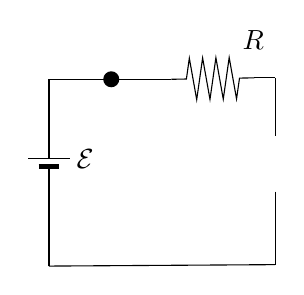
\begin{tikzpicture}[x=0.75pt,y=0.75pt,yscale=-1,xscale=1]
%uncomment if require: \path (0,127); %set diagram left start at 0, and has height of 127

%Straight Lines [id:da24575409936073345] 
\draw    (31,120) -- (139.99,119.3) ;
%Straight Lines [id:da11549410920467973] 
\draw    (31,71) -- (31,120) ;
%Straight Lines [id:da9511010662679844] 
\draw    (31,30) -- (61,30) ;
\draw [shift={(61,30)}, rotate = 0] [color={rgb, 255:red, 0; green, 0; blue, 0 }  ][fill={rgb, 255:red, 0; green, 0; blue, 0 }  ][line width=0.75]      (0, 0) circle [x radius= 3.35, y radius= 3.35]   ;
%Shape: Resistor [id:dp08195888719898736] 
\draw   (90,30) -- (97.2,29.87) -- (98.62,19.85) -- (102.17,39.79) -- (105.02,19.74) -- (108.57,39.68) -- (111.42,19.62) -- (114.97,39.57) -- (117.82,19.51) -- (121.37,39.45) -- (122.8,29.43) -- (129.99,29.3) ;
%Straight Lines [id:da8123208472755747] 
\draw    (139.99,84.17) -- (139.99,119.3) ;
%Straight Lines [id:da27617461873898574] 
\draw    (139.99,29.3) -- (139.99,57.5) ;
%Straight Lines [id:da8813952696008942] 
\draw    (80,30) -- (90,30) ;
%Straight Lines [id:da18537801894992811] 
\draw    (129.99,29.3) -- (139.99,29.3) ;
%Straight Lines [id:da4241233627632246] 
\draw    (21,68) -- (41,68) ;
%Straight Lines [id:da7962359824187548] 
\draw [line width=1.5]    (26,72) -- (36,72) ;
%Straight Lines [id:da5082683737145255] 
\draw    (31,30) -- (31,68) ;
%Straight Lines [id:da8935774178437921] 
\draw    (80,30) -- (61,30) ;

% Text Node
\draw (123,5.4) node [anchor=north west][inner sep=0.75pt]    {$R$};
% Text Node
\draw (43,62.4) node [anchor=north west][inner sep=0.75pt]    {$\mathcal{E}$};


\end{tikzpicture}


Kirchhoff's voltage Law gives

$\mathcal{E}-i(t)R-v_C(t)=0$

For large $t$, $i(t)=0$, leaving $v_{C}(t)=\mathcal{E}$. This voltage is for large $t$, so we relabel it as $V_f$. Using $Q_f=CV_f$ gives $Q_f=C\mathcal{E}$, so

\begin{equation}
q(t)=C\mathcal{E}(1-e^{-t/RC})
\end{equation}

Note that the general formula $q(t)=Q_f(1-e^{-t/\tau})$ that applies for all $t$ is derived by solving the differential equation $\mathcal{E}-i(t)R-v_C(t)=0$ using $i(t)=dq(t)/dt$ and $v_C(t)=Cq(t)$.

\ifsolutions

\else

\newpage
\fi
\ifsolutions\else
\newpage
\fi

\subsection{Problem}

For a circuit with any number of capacitors, DC voltage sources, and resistors, finding the equation for $q(t)$ for each capacitor requires solving a system of differential equations, which is not covered in this course. However, you can find the currents and charges on the capacitor after a long time by replacing all capacitors with open circuits and then using KVL.



\tikzset{every picture/.style={line width=0.75pt}} %set default line width to 0.75pt        

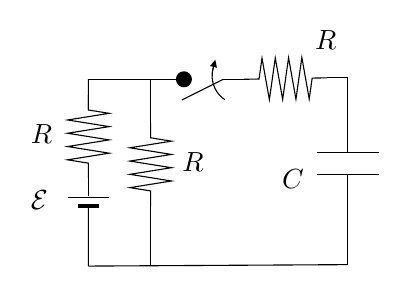
\begin{tikzpicture}[x=0.75pt,y=0.75pt,yscale=-1,xscale=1]
%uncomment if require: \path (0,132); %set diagram left start at 0, and has height of 132

%Straight Lines [id:da5284300597770297] 
\draw    (30,89) -- (30.01,117) ;
%Straight Lines [id:da8080845996289014] 
\draw    (30.01,27) -- (76.01,27) ;
\draw [shift={(76.01,27)}, rotate = 0] [color={rgb, 255:red, 0; green, 0; blue, 0 }  ][fill={rgb, 255:red, 0; green, 0; blue, 0 }  ][line width=0.75]      (0, 0) circle [x radius= 3.35, y radius= 3.35]   ;
%Shape: Resistor [id:dp8493153531836644] 
\draw   (105.01,27) -- (112.2,26.87) -- (113.63,16.85) -- (117.18,36.79) -- (120.03,16.74) -- (123.58,36.68) -- (126.43,16.62) -- (129.98,36.57) -- (132.83,16.51) -- (136.38,36.45) -- (137.8,26.43) -- (145,26.3) ;
%Straight Lines [id:da028128946391895893] 
\draw    (95.01,27) -- (105.01,27) ;
%Straight Lines [id:da2555058455454102] 
\draw    (145,26.3) -- (155,26.3) ;
%Straight Lines [id:da5102685415103501] 
\draw    (20.01,84) -- (40.01,84) ;
%Straight Lines [id:da10033414997314494] 
\draw [line width=1.5]    (25.01,88) -- (35.01,88) ;
%Straight Lines [id:da22873778711306847] 
\draw    (30.01,27) -- (30,41.8) ;
%Straight Lines [id:da6968782624598779] 
\draw    (95.01,27) -- (75.01,37) ;
%Shape: Arc [id:dp23370739223248438] 
\draw  [draw opacity=0] (95.72,36.82) .. controls (93.71,35.49) and (92.03,33.61) .. (90.92,31.27) .. controls (89.42,28.12) and (89.23,24.68) .. (90.12,21.57) -- (103.36,25.36) -- cycle ; \draw   (95.72,36.82) .. controls (93.71,35.49) and (92.03,33.61) .. (90.92,31.27) .. controls (89.42,28.12) and (89.23,24.68) .. (90.12,21.57) ;  
%Straight Lines [id:da8214617203806691] 
\draw    (90.39,20.48) -- (89.83,22.71) ;
\draw [shift={(91.12,17.57)}, rotate = 104] [fill={rgb, 255:red, 0; green, 0; blue, 0 }  ][line width=0.08]  [draw opacity=0] (3.57,-1.72) -- (0,0) -- (3.57,1.72) -- cycle    ;
%Straight Lines [id:da5970328381667953] 
\draw    (30.01,117) -- (155,116.3) ;
%Shape: Resistor [id:dp7636901778703458] 
\draw   (60,48) -- (60,55.2) -- (70,56.8) -- (50,60) -- (70,63.2) -- (50,66.4) -- (70,69.6) -- (50,72.8) -- (70,76) -- (50,79.2) -- (60,80.8) -- (60,88) ;
%Straight Lines [id:da7754838009425478] 
\draw    (60,88) -- (60,117) ;
%Straight Lines [id:da1932685619633996] 
\draw    (60,27) -- (60,55.2) ;
%Straight Lines [id:da5874139525052327] 
\draw    (30,74.6) -- (30,83) ;
%Shape: Resistor [id:dp12780839560321078] 
\draw   (30,34.6) -- (30,41.8) -- (40,43.4) -- (20,46.6) -- (40,49.8) -- (20,53) -- (40,56.2) -- (20,59.4) -- (40,62.6) -- (20,65.8) -- (30,67.4) -- (30,74.6) ;
%Shape: Contact [id:dp33938944783427116] 
\draw   (155,54.2) -- (155,62.2) (155,80.87) -- (155,72.87) (170,62.2) -- (140,62.2) (170,72.87) -- (140,72.87) ;
%Straight Lines [id:da11840524191307011] 
\draw    (155,80.87) -- (155,116) ;
%Straight Lines [id:da9057814699128477] 
\draw    (155,26) -- (155,54.2) ;

% Text Node
\draw (138.01,2.4) node [anchor=north west][inner sep=0.75pt]    {$R$};
% Text Node
\draw (74,61) node [anchor=north west][inner sep=0.75pt]    {$R$};
% Text Node
\draw (1,79.4) node [anchor=north west][inner sep=0.75pt]    {$\mathcal{E}$};
% Text Node
\draw (1,47.4) node [anchor=north west][inner sep=0.75pt]    {$R$};
% Text Node
\draw (122.01,69.1) node [anchor=north west][inner sep=0.75pt]    {$C$};


\end{tikzpicture}


\begin{enumerate}

  \item Find the charge on the capacitor a long time after the switch is closed.

  \item Find the current in the resistor a long time after the switch is closed.

\end{enumerate}

\ifsolutions
\textbf{Answer}

    \begin{enumerate}

      \item $Q_f=\mathcal{E}C$

      \item $i_{Rf}=\mathcal{E}/R$

    \end{enumerate}
\else
\vskip 144pt
\fi
\ifsolutions\else
\vskip 144pt
\fi

\newpage

\section{Charge/Discharge Problem}

\subsection{Part I}



\tikzset{every picture/.style={line width=0.75pt}} %set default line width to 0.75pt        

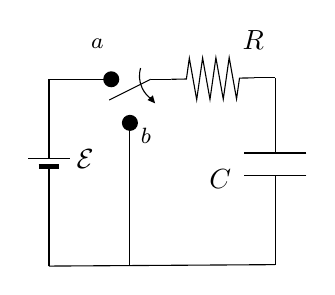
\begin{tikzpicture}[x=0.75pt,y=0.75pt,yscale=-1,xscale=1]
%uncomment if require: \path (0,127); %set diagram left start at 0, and has height of 127

%Straight Lines [id:da9573646957662043] 
\draw    (31,120) -- (139.99,119.3) ;
%Shape: Contact [id:dp9565169725903933] 
\draw   (139.99,57.5) -- (139.99,65.5) (139.99,84.17) -- (139.99,76.17) (154.99,65.5) -- (124.99,65.5) (154.99,76.17) -- (124.99,76.17) ;
%Straight Lines [id:da6284594202215017] 
\draw    (31,71) -- (31,120) ;
%Straight Lines [id:da2136618357878628] 
\draw    (70,51) -- (70,120) ;
\draw [shift={(70,51)}, rotate = 90] [color={rgb, 255:red, 0; green, 0; blue, 0 }  ][fill={rgb, 255:red, 0; green, 0; blue, 0 }  ][line width=0.75]      (0, 0) circle [x radius= 3.35, y radius= 3.35]   ;
%Straight Lines [id:da7490985587148398] 
\draw    (31,30) -- (61,30) ;
\draw [shift={(61,30)}, rotate = 0] [color={rgb, 255:red, 0; green, 0; blue, 0 }  ][fill={rgb, 255:red, 0; green, 0; blue, 0 }  ][line width=0.75]      (0, 0) circle [x radius= 3.35, y radius= 3.35]   ;
%Shape: Resistor [id:dp3525730162875478] 
\draw   (90,30) -- (97.2,29.87) -- (98.62,19.85) -- (102.17,39.79) -- (105.02,19.74) -- (108.57,39.68) -- (111.42,19.62) -- (114.97,39.57) -- (117.82,19.51) -- (121.37,39.45) -- (122.8,29.43) -- (129.99,29.3) ;
%Straight Lines [id:da2977014378130778] 
\draw    (139.99,84.17) -- (139.99,119.3) ;
%Straight Lines [id:da030277022022630495] 
\draw    (139.99,29.3) -- (139.99,57.5) ;
%Straight Lines [id:da11389607646537225] 
\draw    (80,30) -- (90,30) ;
%Straight Lines [id:da24326600748417793] 
\draw    (129.99,29.3) -- (139.99,29.3) ;
%Straight Lines [id:da10435861691939996] 
\draw    (21,68) -- (41,68) ;
%Straight Lines [id:da45732952192697707] 
\draw [line width=1.5]    (26,72) -- (36,72) ;
%Straight Lines [id:da7436885446716952] 
\draw    (31,30) -- (31,68) ;
%Straight Lines [id:da3420346973218358] 
\draw    (80,30) -- (60,40) ;
%Shape: Arc [id:dp5907809839187259] 
\draw  [draw opacity=0] (80.71,39.82) .. controls (78.71,38.49) and (77.02,36.61) .. (75.91,34.27) .. controls (74.42,31.12) and (74.22,27.68) .. (75.11,24.57) -- (88.36,28.36) -- cycle ; \draw   (80.71,39.82) .. controls (78.71,38.49) and (77.02,36.61) .. (75.91,34.27) .. controls (74.42,31.12) and (74.22,27.68) .. (75.11,24.57) ;  
%Straight Lines [id:da6885112532590763] 
\draw    (80.14,39.31) -- (79.71,38.82) ;
\draw [shift={(82.11,41.57)}, rotate = 228.92] [fill={rgb, 255:red, 0; green, 0; blue, 0 }  ][line width=0.08]  [draw opacity=0] (3.57,-1.72) -- (0,0) -- (3.57,1.72) -- cycle    ;

% Text Node
\draw (123,5.4) node [anchor=north west][inner sep=0.75pt]    {$R$};
% Text Node
\draw (107,72.4) node [anchor=north west][inner sep=0.75pt]    {$C$};
% Text Node
\draw (43,62.4) node [anchor=north west][inner sep=0.75pt]    {$\mathcal{E}$};
% Text Node
\draw (50,9.4) node [anchor=north west][inner sep=0.75pt]  [font=\footnotesize]  {$a$};
% Text Node
\draw (74,52.4) node [anchor=north west][inner sep=0.75pt]  [font=\footnotesize]  {$b$};


\end{tikzpicture}


The switch in the above circuit has been in position $a$ for a long time. At $t = 0$, the switch is moved to position $b$. The values of the circuit elements are $\mathcal{E}= 12\text{ V}$, $C = 10\text{ mF}$, and $R = 20\text{ }\Omega$.

Let $t=0^-$ correspond to the time just before the switch is moved from $a$ to $b$. Let $t=0^+$ correspond to the time just after the switch is moved from $a$ to $b$.

\begin{enumerate}

  \item What is the current through the resistor at $t=0^-$?

        \ifsolutions
        \textbf{Answer}: Zero.
        \else
        \vskip 56.25pt
        \fi
        \ifsolutions\else
        \vskip 56.25pt
        \fi

  \item What is the current through the resistor at $t=0^+$?

        \ifsolutions
        \textbf{Answer}: Immediately after the switch is moved to $b$, the capacitor starts to discharge though the resistor. Kirchhoff's Voltage law states that the voltage across the resistor equals the voltage across the capacitor, $v_C$. By Ohm's law current through the resistor is $i(0^+) = v_C(0^+)/R = 12\text{ V}/20\text{ }\Omega = 0.6\text{ A}$.
        \else
        \vskip 56.25pt
        \fi
        \ifsolutions\else
        \vskip 56.25pt
        \fi

  \item What is the charge on the capacitor at $t=0^-$?

        \ifsolutions
        \textbf{Answer}: $q(0^-) = Cv_C(0^-) = (10 \text{ mF})(12\text{ V}) = 120\text{ mC}$.
        \else
        \vskip 56.25pt
        \fi
        \ifsolutions\else
        \vskip 56.25pt
        \fi

  \item What is the charge on the capacitor at $t=0^+$?

        \ifsolutions
        \textbf{Answer}: $120\text{ mC}$
        \else
        \vskip 56.25pt
        \fi
        \ifsolutions\else
        \vskip 56.25pt
        \fi

  \item What is the charge on the capacitor at $t = 200\text{ ms}$?

        \ifsolutions
        {\bf Answer: } The time constant is $RC= (10\text{ mF}) (20\text{ }\Omega) = 200\text{ ms}$. At $t = 200\text{ ms}$, the capacitor is in the process of discharging. The charge on the capacitor varies according to $q(t)=Q_oe^{-t/RC}$, so

        $q(200\text{ ms}) = Q_0e^{-200\text{ ms}/RC} = 120\text{ mC} \cdot e^{-200\text{ ms}/200\text{ ms}} \simeq120\text{ mC}\cdot 0.37 \simeq 44 \text{ mC}$.
        \else
        \vskip 56.25pt
        \fi
        \ifsolutions\else
        \vskip 56.25pt
        \fi

\end{enumerate}

\newpage

\subsection{Part II}



\tikzset{every picture/.style={line width=0.75pt}} %set default line width to 0.75pt        

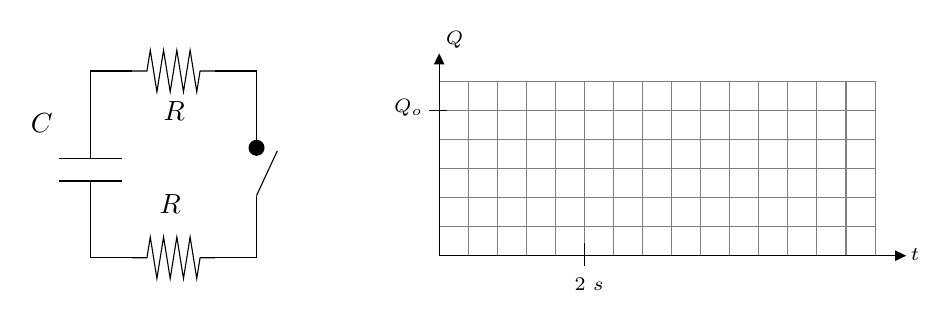
\begin{tikzpicture}[x=0.75pt,y=0.75pt,yscale=-1,xscale=1]
%uncomment if require: \path (0,165); %set diagram left start at 0, and has height of 165

%Straight Lines [id:da12186668018741531] 
\draw    (118,91) -- (118,121) ;
%Straight Lines [id:da5673924877628735] 
\draw    (128,69.5) -- (118,91) ;
%Straight Lines [id:da40110239263509695] 
\draw    (118,31) -- (118,68) ;
\draw [shift={(118,68)}, rotate = 90] [color={rgb, 255:red, 0; green, 0; blue, 0 }  ][fill={rgb, 255:red, 0; green, 0; blue, 0 }  ][line width=0.75]      (0, 0) circle [x radius= 3.35, y radius= 3.35]   ;
%Shape: Grid [id:dp4136213731791418] 
\draw  [draw opacity=0] (206,36) -- (416,36) -- (416,120) -- (206,120) -- cycle ; \draw  [color={rgb, 255:red, 128; green, 128; blue, 128 }  ,draw opacity=1 ] (206,36) -- (206,120)(220,36) -- (220,120)(234,36) -- (234,120)(248,36) -- (248,120)(262,36) -- (262,120)(276,36) -- (276,120)(290,36) -- (290,120)(304,36) -- (304,120)(318,36) -- (318,120)(332,36) -- (332,120)(346,36) -- (346,120)(360,36) -- (360,120)(374,36) -- (374,120)(388,36) -- (388,120)(402,36) -- (402,120)(416,36) -- (416,120) ; \draw  [color={rgb, 255:red, 128; green, 128; blue, 128 }  ,draw opacity=1 ] (206,36) -- (416,36)(206,50) -- (416,50)(206,64) -- (416,64)(206,78) -- (416,78)(206,92) -- (416,92)(206,106) -- (416,106)(206,120) -- (416,120) ; \draw  [color={rgb, 255:red, 128; green, 128; blue, 128 }  ,draw opacity=1 ]  ;
%Straight Lines [id:da6371695008603995] 
\draw [color={rgb, 255:red, 128; green, 128; blue, 128 }  ,draw opacity=1 ]   (206,120) -- (416,120) ;
%Straight Lines [id:da19392406724359912] 
\draw [color={rgb, 255:red, 128; green, 128; blue, 128 }  ,draw opacity=1 ]   (416,120) -- (416,36) ;

%Straight Lines [id:da5115200356999086] 
\draw    (206,25.5) -- (206,120) ;
\draw [shift={(206,22.5)}, rotate = 90] [fill={rgb, 255:red, 0; green, 0; blue, 0 }  ][line width=0.08]  [draw opacity=0] (5.36,-2.57) -- (0,0) -- (5.36,2.57) -- cycle    ;
%Straight Lines [id:da04281112255200381] 
\draw [color={rgb, 255:red, 0; green, 0; blue, 0 }  ,draw opacity=1 ]   (206,120) -- (428,120) ;
\draw [shift={(431,120)}, rotate = 180] [fill={rgb, 255:red, 0; green, 0; blue, 0 }  ,fill opacity=1 ][line width=0.08]  [draw opacity=0] (5.36,-2.57) -- (0,0) -- (5.36,2.57) -- cycle    ;
%Straight Lines [id:da19821580998780153] 
\draw    (276,114) -- (276,125) ;
%Straight Lines [id:da5919180085071085] 
\draw    (210,50) -- (201,50) ;
%Shape: Resistor [id:dp13122071046108608] 
\draw   (58,31) -- (65.2,31) -- (66.8,21) -- (70,41) -- (73.2,21) -- (76.4,41) -- (79.6,21) -- (82.8,41) -- (86,21) -- (89.2,41) -- (90.8,31) -- (98,31) ;
%Straight Lines [id:da48328279530987794] 
\draw    (98,31) -- (118,31) ;
%Shape: Resistor [id:dp9509574212109306] 
\draw   (58,121) -- (65.2,121) -- (66.8,111) -- (70,131) -- (73.2,111) -- (76.4,131) -- (79.6,111) -- (82.8,131) -- (86,111) -- (89.2,131) -- (90.8,121) -- (98,121) ;
%Straight Lines [id:da3895846754264447] 
\draw    (98,121) -- (118,121) ;
%Straight Lines [id:da875812344717507] 
\draw    (38,31) -- (58,31) ;
%Straight Lines [id:da38331316489780587] 
\draw    (38,121) -- (58,121) ;
%Straight Lines [id:da3716022806272685] 
\draw    (38,31) -- (38,65.33) ;
%Shape: Contact [id:dp3229950478101353] 
\draw   (38,65.33) -- (38,73.33) (38,92) -- (38,84) (53,73.33) -- (23,73.33) (53,84) -- (23,84) ;
%Straight Lines [id:da34921956438497426] 
\draw    (38,92) -- (38,121) ;

% Text Node
\draw (8,50.4) node [anchor=north west][inner sep=0.75pt]    {$C$};
% Text Node
\draw (208,10.4) node [anchor=north west][inner sep=0.75pt]  [font=\scriptsize]  {$Q$};
% Text Node
\draw (432,115.4) node [anchor=north west][inner sep=0.75pt]  [font=\scriptsize]  {$t$};
% Text Node
\draw (270,129.4) node [anchor=north west][inner sep=0.75pt]  [font=\scriptsize]  {$2\ s$};
% Text Node
\draw (183,43.4) node [anchor=north west][inner sep=0.75pt]  [font=\scriptsize]  {$Q_{o}$};
% Text Node
\draw (72,44.4) node [anchor=north west][inner sep=0.75pt]    {$R$};
% Text Node
\draw (70,89.4) node [anchor=north west][inner sep=0.75pt]    {$R$};


\end{tikzpicture}


The switch in the above circuit has been in position $b$ for a long time. At $t = 0$, the switch is moved to position $a$. The values of the circuit elements are $\mathcal{E}= 12\text{ V}$, $C = 10\text{ mF}$, and $R = 20\text{ }\Omega$.

Let $t=0^-$ correspond to the time just before the switch is moved from $b$ to $a$. Let $t=0^+$ correspond to the time just after the switch is moved from $b$ to $a$.

\begin{enumerate}

  \item What is the current through the resistor at $t=0^-$?

        \ifsolutions
        {\bf Answer: } Since the switch is on position $b$ for a long time, the charge on and voltage across the capacitor is zero. If the voltage across the capacitor is zero, then by Kirchhoff's voltage law, the voltage across the resistor must be zero. So the current through the resistor is zero.
        \else
        \vskip 56.25pt
        \fi
        \ifsolutions\else
        \vskip 56.25pt
        \fi

  \item What is the voltage across the capacitor at $t=0^-$?

        \ifsolutions
        {\bf Answer: } Zero.
        \else
        \vskip 56.25pt
        \fi
        \ifsolutions\else
        \vskip 56.25pt
        \fi

  \item What is the charge on the capacitor at $t=0^-$?

        \ifsolutions
        {\bf Answer: } Zero.
        \else
        \vskip 56.25pt
        \fi
        \ifsolutions\else
        \vskip 56.25pt
        \fi

  \item What is the charge on the capacitor at  $t=0^+$?

        \ifsolutions
        {\bf Answer: } Zero.
        \else
        \vskip 56.25pt
        \fi
        \ifsolutions\else
        \vskip 56.25pt
        \fi

  \item What is the current through the resistor at $t=0^+$?

        \ifsolutions
        {\bf Answer:} Kirchhoff's voltage law at this time is

        $\mathcal{E}-i(0^+)R-v_C(0^+)=0$

        At $t=0^+$ the voltage across the capacitor is zNeero because it is uncharged, so $i(0^+)R=\mathcal{E}$. Thus, $i(0^+) = \mathcal{E}/R = 12\text{ V}/20\text{ }\Omega = 0.6\text{ A}$.
        \else
        \vskip 56.25pt
        \fi
        \ifsolutions\else
        \vskip 56.25pt
        \fi

  \item What is the charge on the capacitor at time $t = 200\text{ ms}$?

        \ifsolutions
        {\bf Answer: } The time constant is $RC=200\text{ ms}$. At $t=200\text{ ms}$, the charge accumulated on the capacitor is:

        \begin{equation}
        q(200\text{ s}) = C\mathcal{E}(1-e^{-(200\text{ s})/RC}) = (10\text{ mF} \cdot 12\text{ V})(1-e^{-200/200})\simeq (120\text{ mV})(0.63)\simeq 75.9\text{ mV}
        \end{equation}
        \else

        \fi
        \ifsolutions\else

        \fi

\end{enumerate}

\end{document}